\documentclass[class=article, crop=true]{standalone}
\usepackage{subcaption}
\usepackage[subpreambles=true]{standalone}
\usepackage{tikz}
\usepackage{amssymb}
\usepackage{amsmath}
\usetikzlibrary{arrows.meta, positioning}

\begin{document}

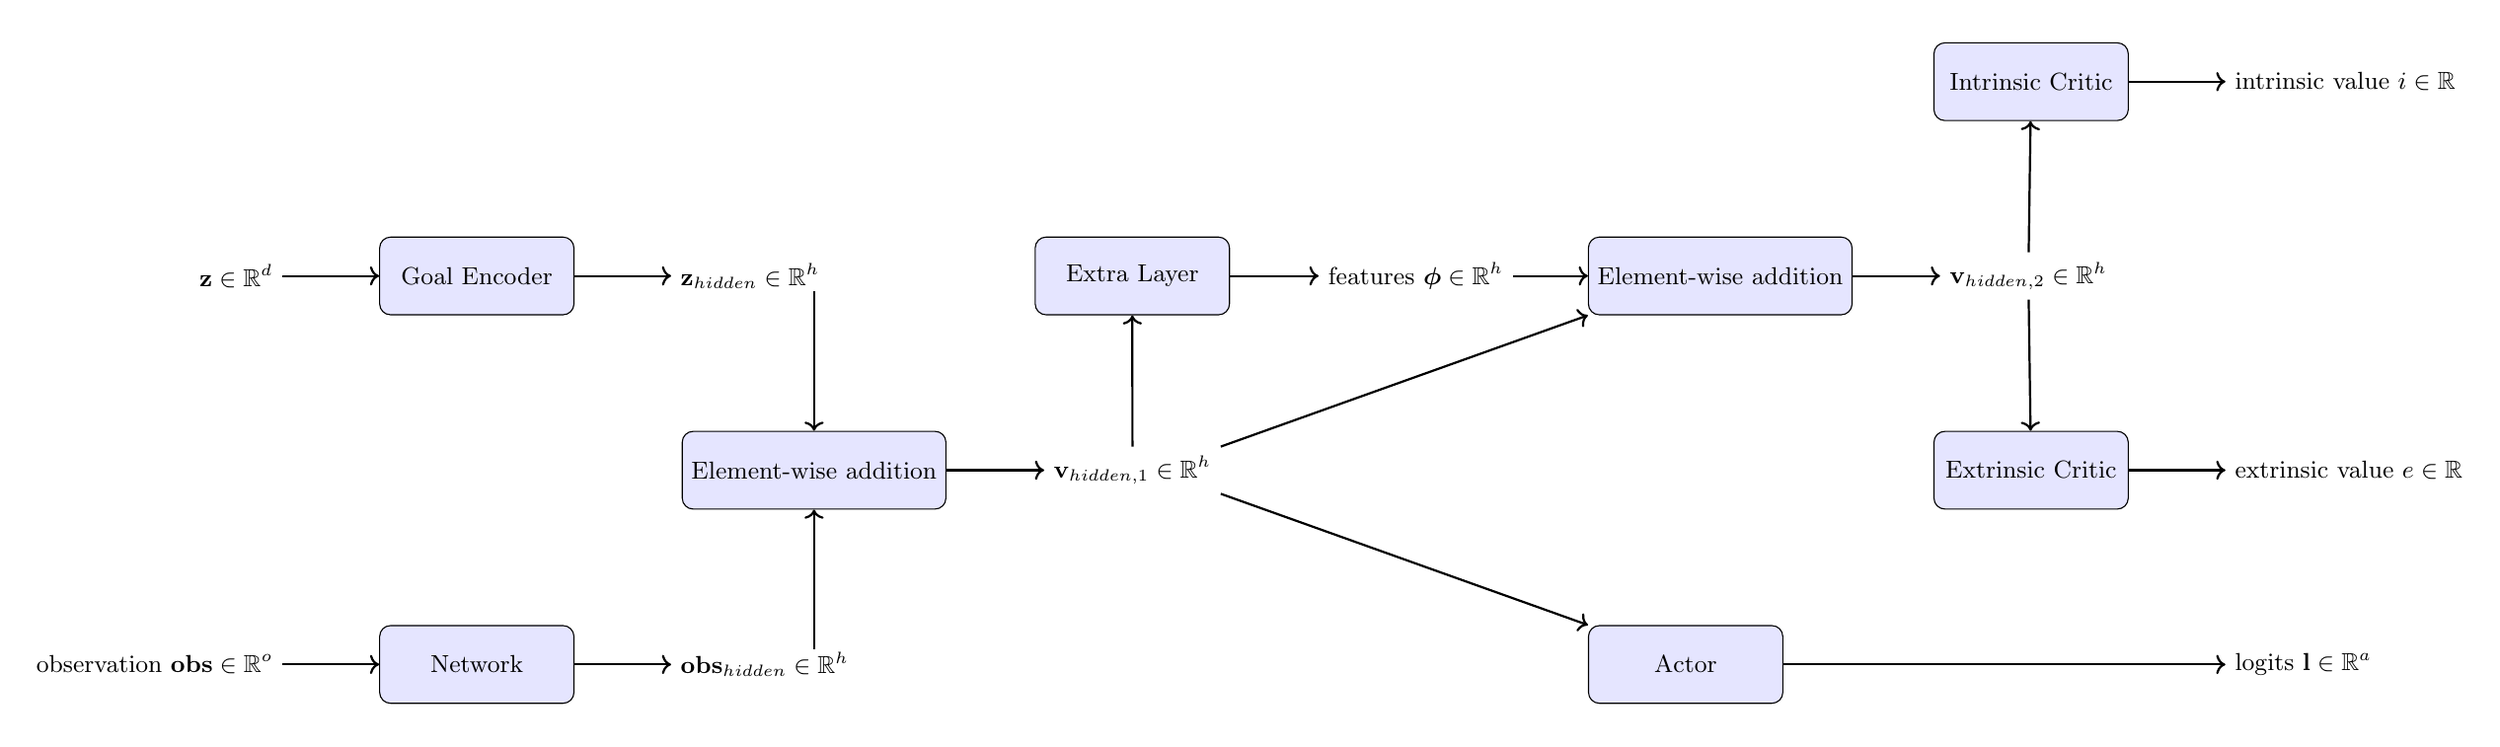
\begin{tikzpicture}[
    op/.style={rectangle, draw, rounded corners, text centered, minimum height=1cm, minimum width=2.5cm, font=\small, fill=blue!10},
    %tensor/.style={font=\small, text centered},
    tensor/.style={font=\small},
    arrow/.style={->, thick},
    %node distance=0.8cm and 1.2cm % Compact spacing
]

%Background
\fill[white] (-13.2, -3.2) rectangle (18.1, 5.7);

% Input nodes
%\node[tensor] (obs) {observation $\in \R^o$};
%\node[tensor, right=of obs] (goal) {z $\in \R^d$};

\node[tensor, anchor=east] (obs) at (-10, -2.5) {observation $\textbf{obs} \in \mathbb{R}^o$};
\node[tensor, anchor=east] (goal) at (-10, 2.5) {$\textbf{z} \in \mathbb{R}^d$};

% Hidden layers
%\node[op, below=of obs] (network) {Network};
%\node[op, below=of goal] (goal_encoder) {Goal Encoder};

%\node[tensor, below=of network] (obs_hidden) {observation hidden $\in \R^h$};
%\node[tensor, below=of goal_encoder] (goal_hidden) {z hidden $\in \R^h$};

\node[op] (network) at (-7.5, -2.5) {Network};
\node[op] (goal_encoder) at (-7.5, 2.5) {Goal Encoder};

\node[tensor, anchor=west] (obs_hidden) at (-5, -2.5) {$\textbf{obs}_{hidden} \in \mathbb{R}^h$};
\node[tensor, anchor=west] (goal_hidden) at (-5, 2.5) {$\textbf{z}_{hidden} \in \mathbb{R}^h$};

% Element-wise addition 1
%\node[op, below=of obs_hidden, xshift=1.5cm] (element_wise_addition_1) {Element-wise addition};
%\node[tensor, below=of element_wise_addition_1] (hidden) {hidden $\in \R^h$};

\node[op] (element_wise_addition_1) at (-3.16, 0) {Element-wise addition};
\node[tensor, anchor=west] (hidden) at (-0.2, 0) {$\textbf{v}_{hidden, 1} \in \mathbb{R}^h$};

% Actor Branch
%\node[op, below left=of hidden] (actor) {Actor};
%\node[tensor, below=of actor] (logits) {logits $\in \R^a$};

\node[op] (actor) at (8.055, -2.5) {Actor};
\node[tensor, anchor=west] (logits) at (15, -2.5) {logits $\textbf{l} \in \mathbb{R}^a$};

% Extra Layer Branch
%\node[op, right=2cm of hidden] (extra_layer) {Extra Layer};
%\node[tensor, below=of extra_layer] (features) {features $\in \R^h$};
%\node[op, below=of features] (element_wise_addition_2) {Element-wise addition};
%\node[tensor, below=of element_wise_addition_2] (hidden_2) {hidden 2 $\in \R^h$};

\node[op] (extra_layer) at (0.935, 2.5) {Extra Layer};
\node[tensor, anchor=west] (features) at (3.332, 2.5) {features $\boldsymbol{\phi} \in \mathbb{R}^h$};
\node[op] (element_wise_addition_2) at (8.5, 2.5) {Element-wise addition};
\node[tensor, anchor=west] (hidden_2) at (11.328, 2.5) {$\textbf{v}_{hidden, 2} \in \mathbb{R}^h$};

% Critic Branch
%\node[op, below left=of hidden_2] (critic_ext) {Extrinsic Critic};
%\node[tensor, below=of critic_ext] (value_ext) {extrinsic value $\in \R$};
%\node[op, below right=of hidden_2] (critic_int) {Intrinsic Critic};
%\node[tensor, below=of critic_int] (value_int) {intrinsic value $\in \R$};

\node[op] (critic_ext) at (12.5, 0) {Extrinsic Critic};
\node[tensor, anchor=west] (value_ext) at (15, 0) {extrinsic value $e \in \mathbb{R}$};
\node[op] (critic_int) at (12.5, 5) {Intrinsic Critic};
\node[tensor, anchor=west] (value_int) at (15, 5) {intrinsic value $i \in \mathbb{R}$};

% Arrows
\draw[arrow] (obs) -- (network);
\draw[arrow] (goal) -- (goal_encoder);
\draw[arrow] (network) -- (obs_hidden);
\draw[arrow] (goal_encoder) -- (goal_hidden);
%\draw[arrow] (obs_hidden) -- (element_wise_addition_1);
%\draw[arrow] (goal_hidden) -- (element_wise_addition_1);
\draw[arrow] (-3.16, -2.3) -- (element_wise_addition_1.south);
\draw[arrow] (-3.16, 2.3) -- (element_wise_addition_1.north);
\draw[arrow] (element_wise_addition_1) -- (hidden);

% Actor Branch
\draw[arrow] (hidden.south east) -- (actor.north west);
\draw[arrow] (actor) -- (logits);

% Extra Layer Branch
\draw[arrow] (hidden) -- (extra_layer);
\draw[arrow] (hidden.north east) -- (element_wise_addition_2.south west); % Connection preserved
\draw[arrow] (extra_layer) -- (features);
\draw[arrow] (features) -- (element_wise_addition_2);
\draw[arrow] (element_wise_addition_2) -- (hidden_2);

% Critic Branch
\draw[arrow] (hidden_2) -- (critic_ext);
\draw[arrow] (hidden_2) -- (critic_int);
\draw[arrow] (critic_ext) -- (value_ext);
\draw[arrow] (critic_int) -- (value_int);

\end{tikzpicture}

\end{document}
